\section{System's Perspective} \label{sec:system}
This section documents the architecture of the MiniTwit application. We will describe the individual dependencies of the application and why we choose them. We will also describe what the current state of the system is.

\subsection{Architecture \& Design}
The MiniTwit application relies on a lot of dependencies, which interact with each other in many ways. Figure \ref{fig:architecture} shows all of these interactions. In figure \ref{fig:architecture} it can be seen that a pipeline of actions is initiated every time someone commits to the MiniTwit GitHub repository. When someone commits a change, the GitHub Actions initialize our CI/CD setup, which is described in section \ref{sec:cicd}. This setup deploys the image of the application and all it's dependencies, which are described in section \ref{sec:dependencies}, to the Docker Hub. From the Docker Hub, everything is deployed to DigitalOcean which hosts our application. On DigitalOcean we use a replication setup, described in section \ref{sec:scaling}, which ensures availability of the application.

\begin{figure}[H]
    \centering
    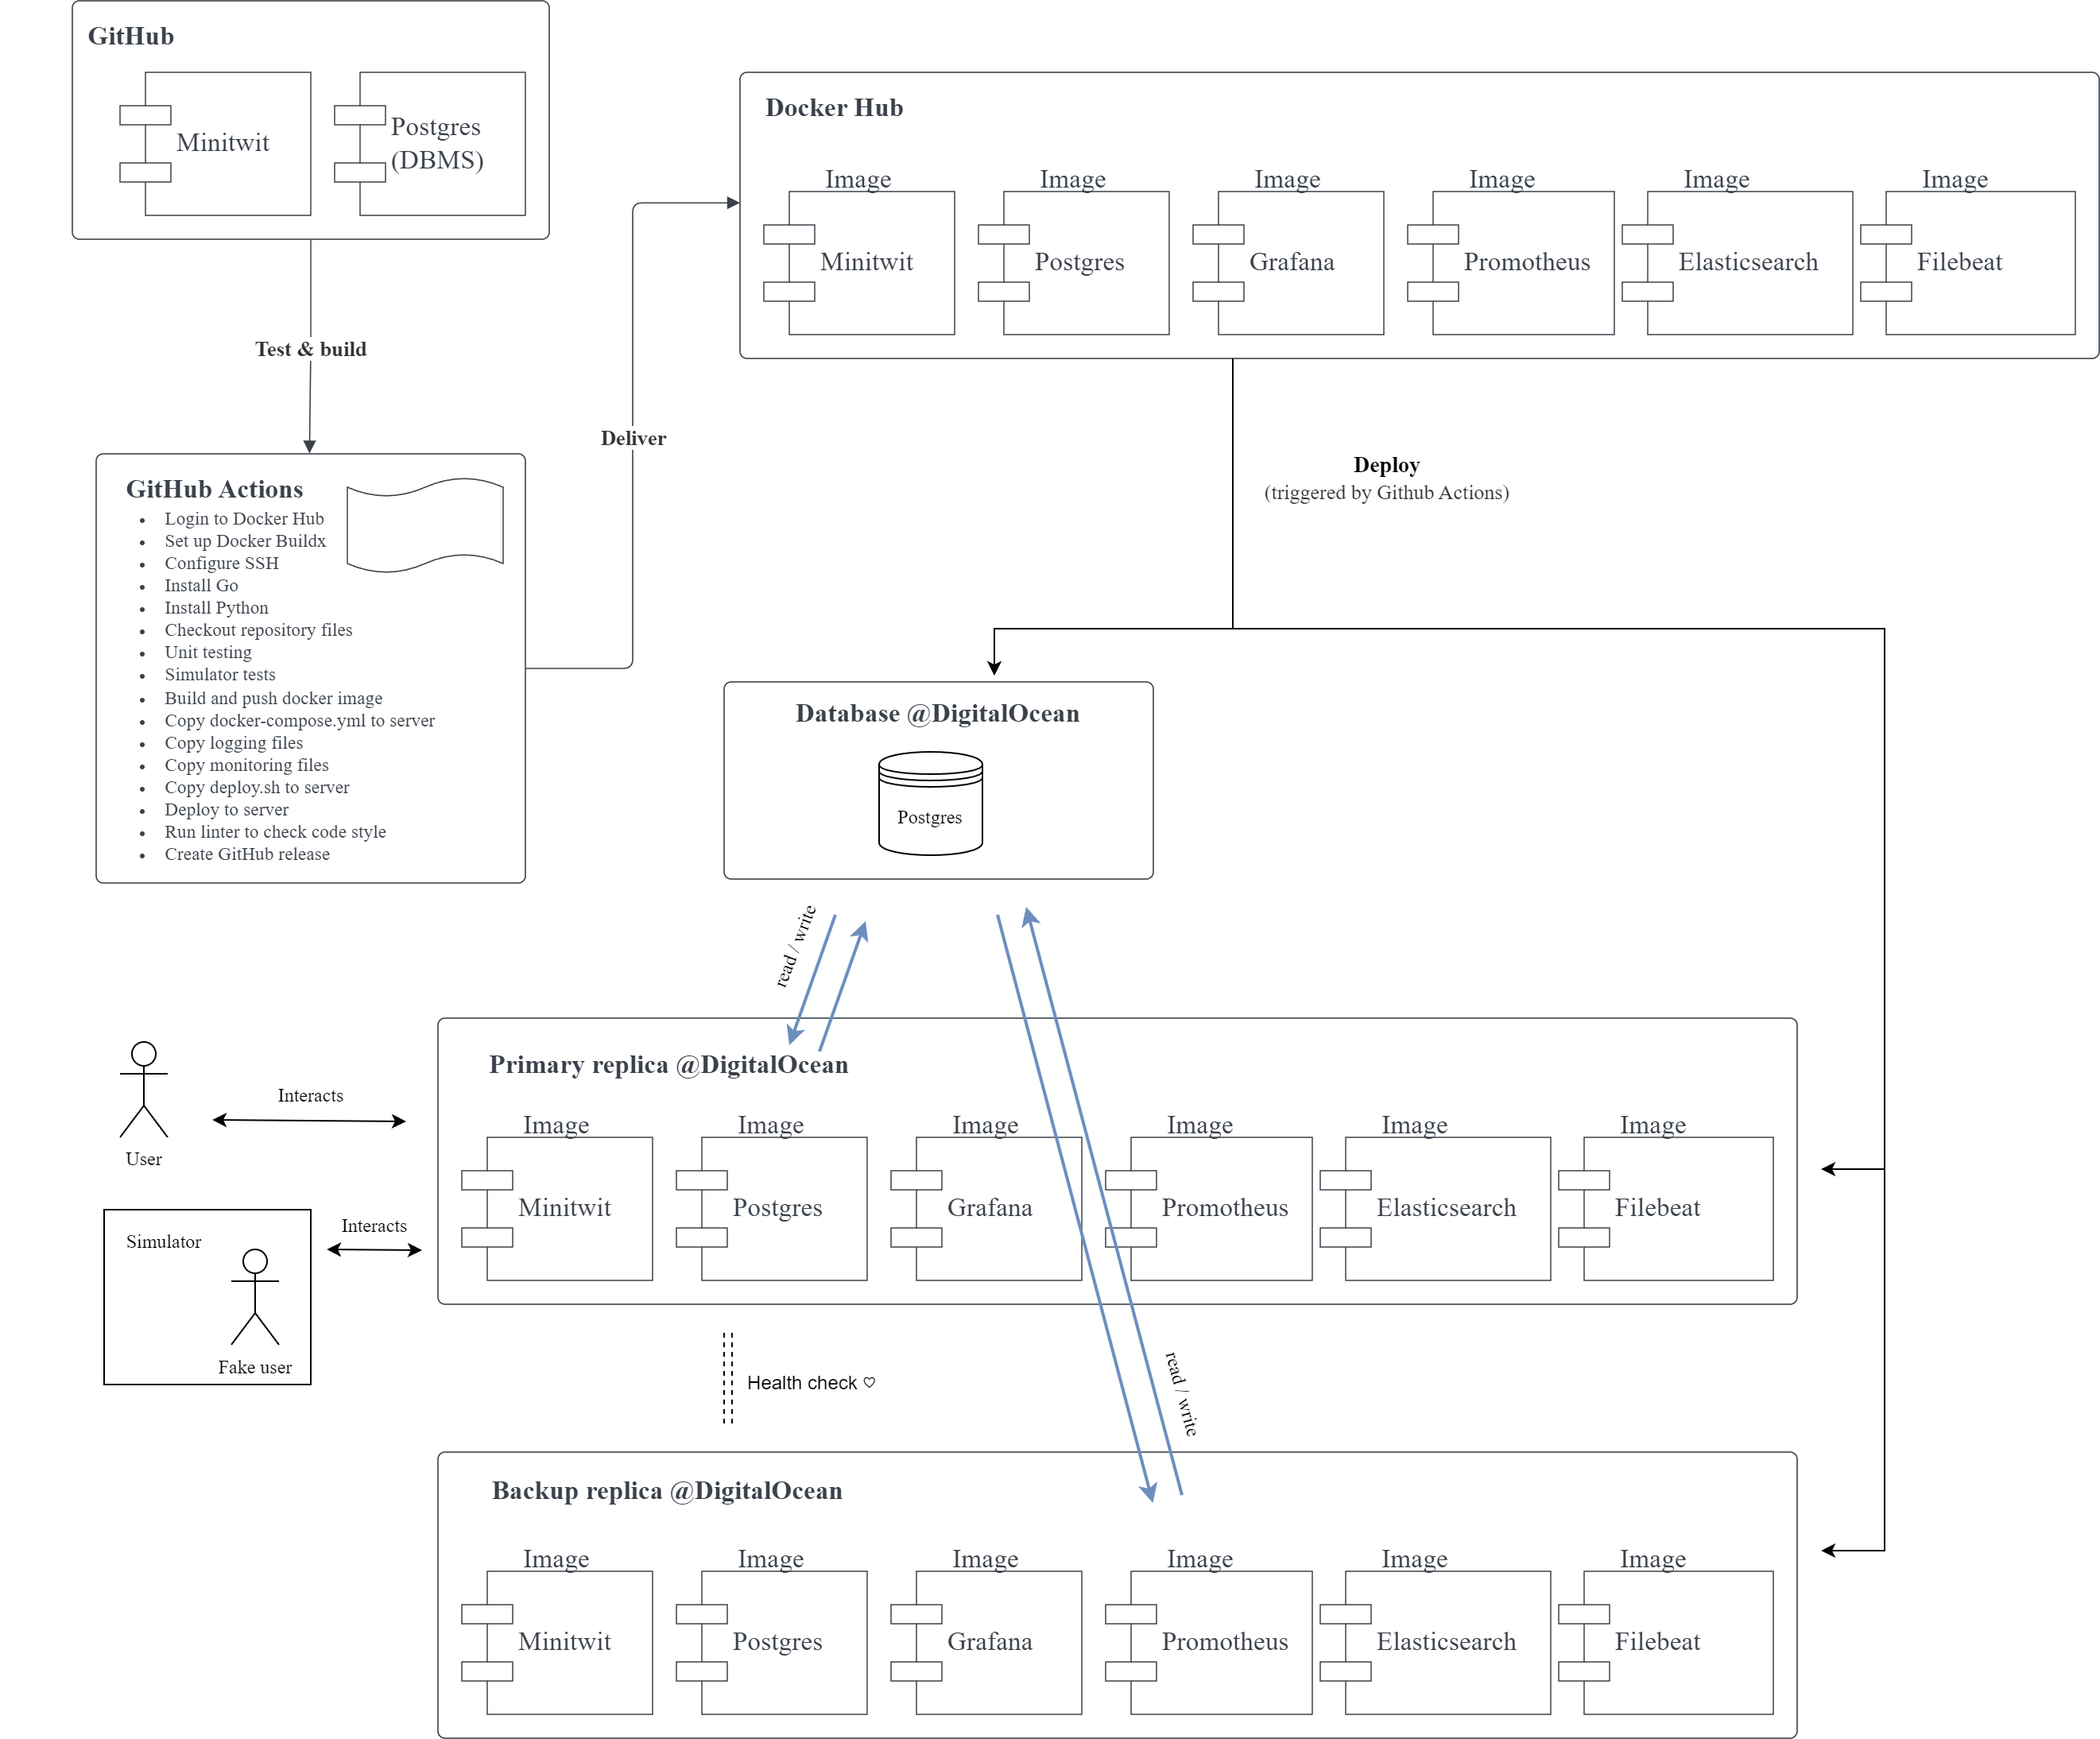
\includegraphics[width=\linewidth]{images/architecture.png}
    \caption{Architecture of the MiniTwit application. The diagram shows which dependencies are involved in the application, and how they interact with each other.}
    \label{fig:architecture}
\end{figure}

\subsection{Dependencies} \label{sec:dependencies}
%arguments for choice of technologies
This section describes the different dependencies used in our application, and we argue for the choice of each technology.

\paragraph*{Docker}
We use Docker\footnote{\href{https://www.docker.com/}{docker.com}} to containerize all of our dependencies, into convenient images which are far easier to transport and deploy. Without utilizing containerization, like Docker offers, it would be a struggle to keep track of every tool we use and all the technologies their depend on, and it would require a lot of steps every time we would have to run our application. Docker allows us to package everything together, and lets us run everything from one single command. The reason for using Docker, over other containerization tools such as Kubernetes, is because we already have experience using Docker from previous courses, and because it offers all the functionality we need for our application.

\paragraph*{Go \& Gin}
We choose to utilize Gin\footnote{\href{https://gin-gonic.com/}{gin-gonic.com}} for our web-application. Gin is an web framework written in Go/Golang, which allows for development of fast and stable web services. We choose to use Gin as it's faster than many other web development frameworks, including Flask which is the original framework that the MiniTwit application was using. We wanted our web framework to support HTML rendering, and to support the use of relational databases, as we wanted to be able to reuse as much of the original MiniTWit application as possible. Gin supports both of these features while being scalable and offering type safety, which is important for writing maintainable code, and therefore we though that Gin was very suitible for our MiniTwit application. Additionally we also saw this project as an perfect opportunity to learn Go, and to use Gin.

\paragraph*{Gorm}
In Go, one of the most popular ORM libraries is Gorm\footnote{\href{https://gorm.io/}{gorm.io}}. We chose this library because it is one of the most mature libraries we could choose out of the possible ones for Go. Gorm has the basic ORM features we needed like creation, update, and deletion of database objects. With Gorm we could create objects in Go that has the fields needed for the database.

\paragraph*{Vagrant}
\paragraph*{Prometheus \& Grafana}
\paragraph*{Elasticsearch, Filebeat \& Kibana}
To facilitate logging in our Minitwit application, we decided to implement an EFK stack. The EFK stack is a great fit for our Minitwit application as it provides a lightweight log shipper in Filebeat which can collect logs from the application, parse them and forward them to a storage component. It provides an efficient storage and analytics engine in Elastic search, which enables efficient handling of large data volumes and is excellent for full-text search. Lastly, it provides a simple to setup dashboard in Kibana that allows for filtering queries on the data stores in elastic search, such that we only display the data that we find most valuable. 

\paragraph*{DigitalOcean}
We have DigitalOcean as our cloud infrastructure provider. DigitalOcean offers a user-friendly interface for setting up and deploying Droplets (VMs) and Volumes (storage). In general, it is known for its simplicity and affordability which makes it ideal for our Minitwit application.

\paragraph*{Github \& GH Actions}
To facilitate our CI/CD workflow we utilize GitHub Actions because it is integrated in GitHub, which is the version control system we use for our repository. This way we don't have to involve other platforms, and we can keep everything in one place. Also, since it is integrated in GitHub, we can see the status of individual commits when we push them. This way we can see whether individual commits build (or contain errors), and we can see whether individual commits pass tests. Lastly, it allows for Continuous Delivery and Deployment, which means we can automate the delivery or deployment of our changes all with the same system.


%Check the licenses are compatible

\subsection{Current state of the system}

%license included